\chapter{Аналитическая часть}

В данном разделе рассматривается система, в которой происходит волновой процесс, состоящая из поверхности воды и предмета. Изучаются и сравниваются методы и алгоритмы, визуализирующие волны. В результате анализа определяется алгоритм, эффективно решающий задачу моделирования волн, образованных движением объекта.

\section{Волновой процесс}

Процесс образования волны при условии, что частицы воды находятся в состоянии равновесия, состоит из следующих этапов:

\begin{itemize}
	\item на поверхность воды оказывается внешнее воздействие (ветер, движение корабля, падение камня), частицы жидкости опускаются вниз, водная поверхность становится вогнутой;
	\item сила тяжести или сила поверхностного натяжения стремятся вернуть частицы в состояние равновесия;
	\item частицы воды переходят положения равновесия, и поверхность воды становится выпуклой.
\end{itemize}

Движение передается от одних частиц к другим. Этапы волнового процесса показаны на рисунке \ref{img:wave-process}.

\begin{figure}[H]
	\begin{center}
		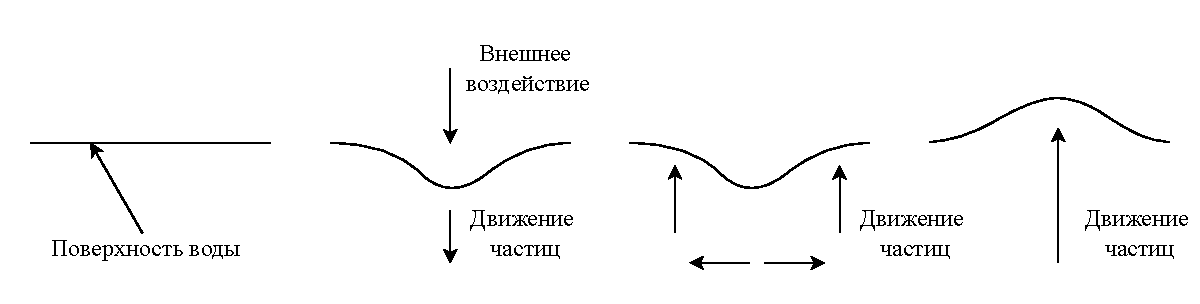
\includegraphics[scale=0.8]{img/wave-process.pdf}
	\end{center}
	\captionsetup{justification=centering}
	\caption{Процесс образования волны}
	\label{img:wave-process}
\end{figure}

Если восстановить равновесие стремится сила тяжести, то волны называются гравитационными, если сила поверхностного натяжения --- капиллярными. Волны называют капиллярно-гравитационными, когда силы сопоставимы.

\section{Модели предмета и волны}

Внешним воздействием в моделируемой системе является движение предмета.

\subsection{Модель предмета}

Для правильной обработки появления волн от твердого тела важны параметры только той части предмета, которая касается воды. В связи с этим нет необходимости рассматривать объект детально.

\subsection{Модель волны}

Геометрически волна состоит из следующих элементов:

\begin{itemize}
	\item гребень --- множество точек волны с максимальным положительным отклонением от состояния равновесия;
	\item подошва --- множество точек волны с наибольшим отрицательным отклонением от состояния равновесия.
\end{itemize}

Кроме того волна обладает следующими параметрами:

\begin{itemize}
	\item высота --- вертикальное расстояние от подошвы до гребня;
	\item длина --- горизонтальное расстояние от гребня до гребня;
	\item период --- временной интервал между прибытием последовательных гребней;
	\item частота --- величина, обратная периоду;
	\item амплитуда --- максимальное отклонение точек волны от положения равновесия;
	\item скорость распространения.
\end{itemize}

Модель волны показана на рисунке \ref{img:wave}.

\begin{figure}[H]
	\begin{center}
		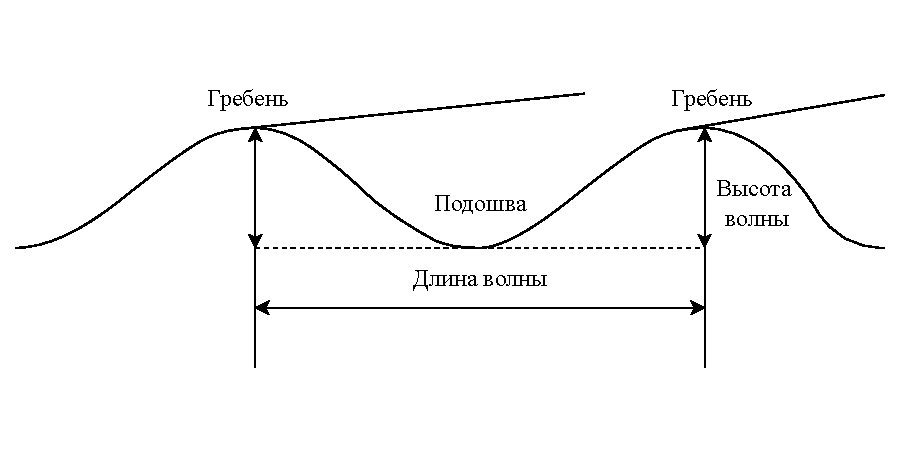
\includegraphics[scale=0.8]{img/wave.pdf}
	\end{center}
	\captionsetup{justification=centering}
	\caption{Геометрическое строение волны}
	\label{img:wave}
\end{figure}

Параметры волны, показанные на рисунке \ref{img:math-wave}, обозначаются следующим образом:

\begin{itemize}
	\item $h(x,t)$ --- высота волны в положении $x$ в момент времени $t$;
	\item $\lambda$ --- длина;
	\item $T$ --- период;
	\item $\nu$ --- частота;
	\item $A$ --- амплитуда;
	\item $v$ --- скорость распространения.
\end{itemize}

\begin{figure}[H]
	\begin{center}
		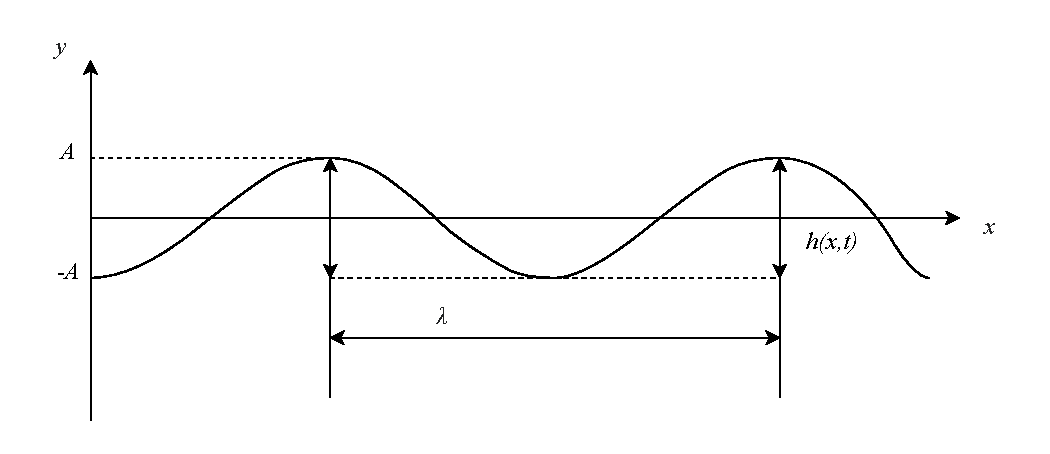
\includegraphics[scale=0.8]{img/math-wave.pdf}
	\end{center}
	\captionsetup{justification=centering}
	\caption{График распространения волны}
	\label{img:math-wave}
\end{figure}

Распространение волн в среде в общем случае описывается волновым уравнением:

\begin{equation}
    \label{wave-eq}
    \Delta h(x,t) = \frac{1}{v^2} \cdot \frac{\partial ^2h(x,t)}{\partial t^2}
\end{equation}

где $\Delta$ --- оператор Лапласа, $x \in \mathbb{R}^2$. 

Решением волнового уравнения \ref{wave-eq} является уравнение бегущей волны:

\begin{equation}
    \label{solution-wave-eq1}
    h(x,t) = A \cos \omega (t - \frac{x}{v})
\end{equation}

где $\omega$ - циклическая частота, которая равняется

\begin{equation}
    \label{w}
    \omega = 2\pi \nu
\end{equation}

Можно ввести волновое число:

\begin{equation}
    \label{k1}
    k = \frac{2\pi}{\lambda}
\end{equation}

Длину волны $\lambda$ можно выразить следующей формулой:

\begin{equation}
    \label{l}
    \lambda = vT
\end{equation}

С учетом формул \ref{w} и \ref{l} формулу \ref{k1} можно записать так:

\begin{equation}
    \label{k2}
    k = \frac{2\pi}{vT} = \frac{2\pi \nu}{v} = \frac{\omega}{v}
\end{equation}

Отсюда скорость распространения волны:

\begin{equation}
    \label{speed}
    v = \frac{\omega}{k}
\end{equation}

Тогда уравнение бегущей волны \ref{solution-wave-eq1}:

\begin{equation}
    \label{solution-wave-eq2}
    h(x,t) = A \cos \omega (t - \frac{x}{v}) = A \cos (\omega t - \omega \frac{kx}{\omega}) = A \cos (\omega t - kx)
\end{equation}

При поглощении средой энергии волны наблюдается затухание волн. Поэтому уравнение бегущей волны принимает вид:

\begin{equation}
    \label{solution-wave-eq3}
    h(x,t) = A \exp(-\beta t) \cos (\omega t - kx)
\end{equation}

где $\beta$ --- коэффициент затухания.

\section{Дисперсионное соотношение}

Механизм образования волн подчиняется закону дисперсии.

Дисперсия волн --- это зависимость циклической частоты волны от волнового вектора:

\begin{equation}
    \label{dispersion}
    \omega = \omega (k)
\end{equation}

Соотношение означает, что волны разных длин перемещаются с разными фазовыми скоростями. Именно дисперсия создает сложную картину волн, образованных телом в воде.

В зависимости от требований к результату моделирования выбирается определенный метод визуализации. Так как в центре работы дисперсионные волны, для выполненения поставленных задач необходим такой метод моделирования, при котором выполняется дисперсионное соотношение.

\section{Методы визуализации волн}

Существует три группы методов моделирования волн:

\begin{itemize}
    \item процедурные;
    \item методы на основе частиц;
    \item метод поля высоты.
\end{itemize}

\subsection{Процедурные методы}

Идея процедурных методов заключается в представлении волновой поверхности наложением периодических функций: циклоиды в ранних работах и синусоиды в дальнейших. 

\begin{figure}[H]
	\begin{center}
		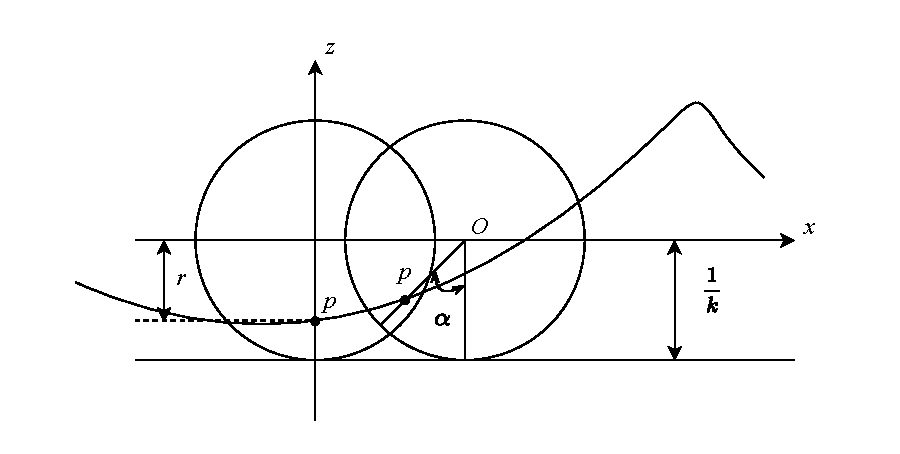
\includegraphics[scale=0.8]{img/procedure.pdf}
	\end{center}
	\captionsetup{justification=centering}
	\caption{Движение точки в процедурном методе}
	\label{img:procedure}
\end{figure}

На рисунке \ref{img:procedure} плоскость покоящейся волновой поверхности параллельна плоскости $XY$, ось $Z$ направлена вверх. Точка $p$ описывает окружность радиусом $\frac{1}{k}$ вокруг своего положения покоя --- точки $O$ с координатами $(x_{O}, y_{O}, z_{O})$. Точка $p$ находится на расстоянии $r$ от точки $O$. Тогда уравнение движения точки:

\begin{equation}
    \label{x}
    x = x_{O} + r\sin (kx_{O} - \omega t)
\end{equation}

\begin{equation}
    \label{z}
    z = z_{O} - r\cos (kx_{O} - \omega t)
\end{equation}

Волна --- траектория движения точки $p$. Для создания различных волновых эффектов изменяют параметры уравнений орбиты, например, радиус или фазовый угол $\alpha$.

Преимущество процедурных методов --- возможность точно контролировать движение волнового спектра.

Недостаток процедурных методов --- сложность получения правильного взаимодействия волн с погруженными телами и границами.  

\subsection{Методы на основе частиц}

В методах моделирования волновой поверхности на основе частиц вода представляется как система частиц. Каждая частица $i$ имеет массу $m_{i}$ и обладает плотностью $\rho _{i}$, давлением $p_{i}$ и объемом $V_{i}$. С течением времени $t$ положение частицы $x_{i}$ и ее параметры меняются в соответствии с учетом скорости $v_{i}$:

\begin{equation}
    \label{vi}
    \frac{dx_{i}}{dt} = v_{i}
\end{equation}

Частицы движутся в потоке жидкости, поэтому скорость $v_{i}$ определяется формой Лагранжа уравнения Навье-Стокса:

\begin{equation}
    \label{dv}
    \frac{dv_{i}}{dt} = -\frac{1}{\rho _{i}} \nabla p_{i} + \nu \nabla ^2 v_{i} + \frac{F_{i}}{m_{i}}.
\end{equation}

где $\nu$ --- вязкость, $-\frac{1}{\rho _{i}} \nabla p_{i}$ описывает ускорение частиц из-за давления в жидкости, $\nu \nabla ^2 v_{i}$ --- ускорение, обсуловленное силами трения между частицами с разными скоростями, $\frac{F_{i}}{m_{i}}$ --- другие ускорения, например ускорение свободного падения.

\begin{figure}[H]
	\begin{center}
		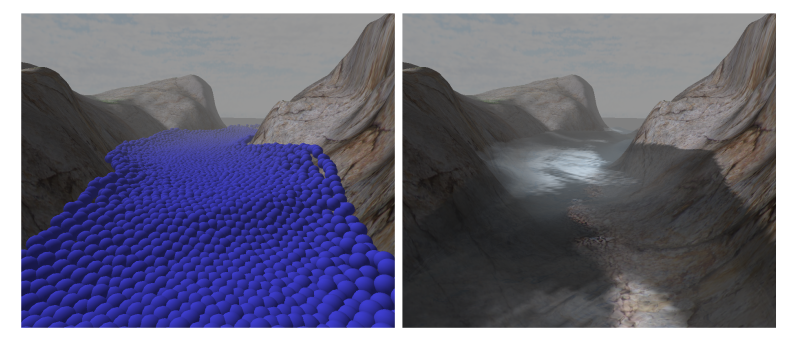
\includegraphics[scale=0.5]{img/particle.png}
	\end{center}
	\captionsetup{justification=centering}
	\caption{Моделирование при помощи метода на основе частиц}
	\label{img:particle}
\end{figure}

Число частиц интерполируется при помощи сглаживающей функции, которая является кубическим сплайном.

Преимущество методов на основе частиц --- возможность добавлять и удалять расчетные точки во время моделирования.

Недостатки методов на основе частиц:
\begin{itemize}
	\item необходимость большого числа частиц для создания реалистичного изображения;
	\item создание неточных границ при контакте жидкости с твердым предметом или другой жидкостью.
\end{itemize} 

\subsection{Метод поля высоты}

В методе поля высоты рассматривают волновое уравнение \ref{wave-eq}. Волновая поверхность представляется в виде двумерной функции --- поля высоты. Такое упрощение снижает вычислительные затраты. Поверхность дискретизируется в сетку, показанную на рисунке \ref{img:grid}, и определяется приблизительное решение в каждой точке сетки.

\begin{figure}[H]
	\begin{center}
		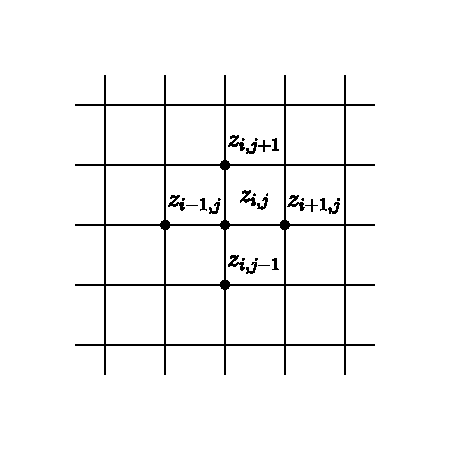
\includegraphics[scale=0.9]{img/grid.pdf}
	\end{center}
	\captionsetup{justification=centering}
	\caption{Представление волновой поверхности в виде сетки}
	\label{img:grid}
\end{figure}

Значение функции $h(x_{i,j})$ в точке сетки с координатам $(i,j)$ обозначается $z_{i,j}$. Оператор Лапласа в волновом уравнении:

\begin{equation}
    \label{laplace1}
    \Delta h(x_{i,j}) \approx \frac{z_{i+1,j} - 2z_{i,j} + z_{i-1,j}}{H^2} + \frac{z_{i,j+1} - 2z_{i,j} + z_{i,j-1}}{H^2}
\end{equation}

\begin{equation}
    \label{laplace2}
    \Delta h(x_{i,j}) = \frac{z_{i+1,j} + z_{i,j+1} - 4z_{i,j} + z_{i-1,j} + z_{i,j-1}}{H^2}
\end{equation}

где $H$ --- расстояние между двумя точками сетки.

Дискретизация времени обозначается $\Delta t$, значение точки с координатами $(i,j)$ в момент времени $t$ --- $z^t_{i,j}$. Тогда производная по времени в волновом уравнении:

\begin{equation}
    \label{second-derivative}
    \frac{\partial ^2h(x,t)}{\partial t^2} \approx \frac{z^{t+1}_{i,j} - 2z^t_{i,j} + z^{t-1}_{i,j}}{\Delta t^2}
\end{equation}

С учетом \ref{laplace2} и \ref{second-derivative} решение волнового уравнения:

\begin{equation}
    \label{1}
    \Delta h(x,t) - \frac{1}{v^2} \cdot \frac{\partial ^2h(x,t)}{\partial t^2} = 0
\end{equation}

\begin{equation}
    \label{2}
    \frac{z_{i+1,j} + z_{i,j+1} - 4z_{i,j} + z_{i-1,j} + z_{i,j-1}}{H^2} - \frac{1}{v^2} \frac{z^{t+1}_{i,j} - 2z^t_{i,j} + z^{t-1}_{i,j}}{\Delta t^2}
\end{equation}

\begin{equation}
    \label{3}
    z^{t+1}_{i,j} = \frac{v^2 \Delta t^2}{H^2} \cdot (z^t_{i+1,j} + z^t_{i,j+1} + z^t_{i-1,j} + z^t_{i,j-1}) + (2-4\frac{v^2 \Delta t^2}{H^2}) \cdot z^t_{i,j} - z^ {t-1}_{i,j}
\end{equation}

Преимущества метода поля высоты:

\begin{itemize}
	\item повышение скорости моделирования;
	\item точность обработки взаимодействия с препятствиями.
\end{itemize}

Недостатком метода поля высоты является невозможность создания обрушивающихся волн  из-за одинаковой скорости распространения всех волн.

Комбинация методов поля высоты и методов, основанных на частицах, позволяет обходить недостатки отдельных и создавать различные эффекты.

\section*{Вывод}

Процедурные методы и методы на основе частиц имеют сложности при работе с твердыми телами. Метод поля высот корректно обрабатывает взаимодействие с объектом, причем с более высокой скоростью моделирования. Недостатки метода поля высот не имеют значения при решении выбранной задачи. Моделирование волн будет реализовано при помощи метода поля высот.

\section{Методы рендеринга отображения}

TODO

\section{Существующие программные обеспечения}

Одним из популярных программных обеспечений для моделирования жидкости, в том числе и волн, является расширение Blender --- Mantaflow. В этом программном продукте существует возможность реализовать моделирование линейных волн, гибкие системы частиц, различные эффекты для жидкости, например, поверхностную турбулентность и вейвлет (небольшую рябь). На рисунке \ref{img:mantaflow} показано моделирование волн в Mantaflow. 

\begin{figure}[H]
	\begin{center}
		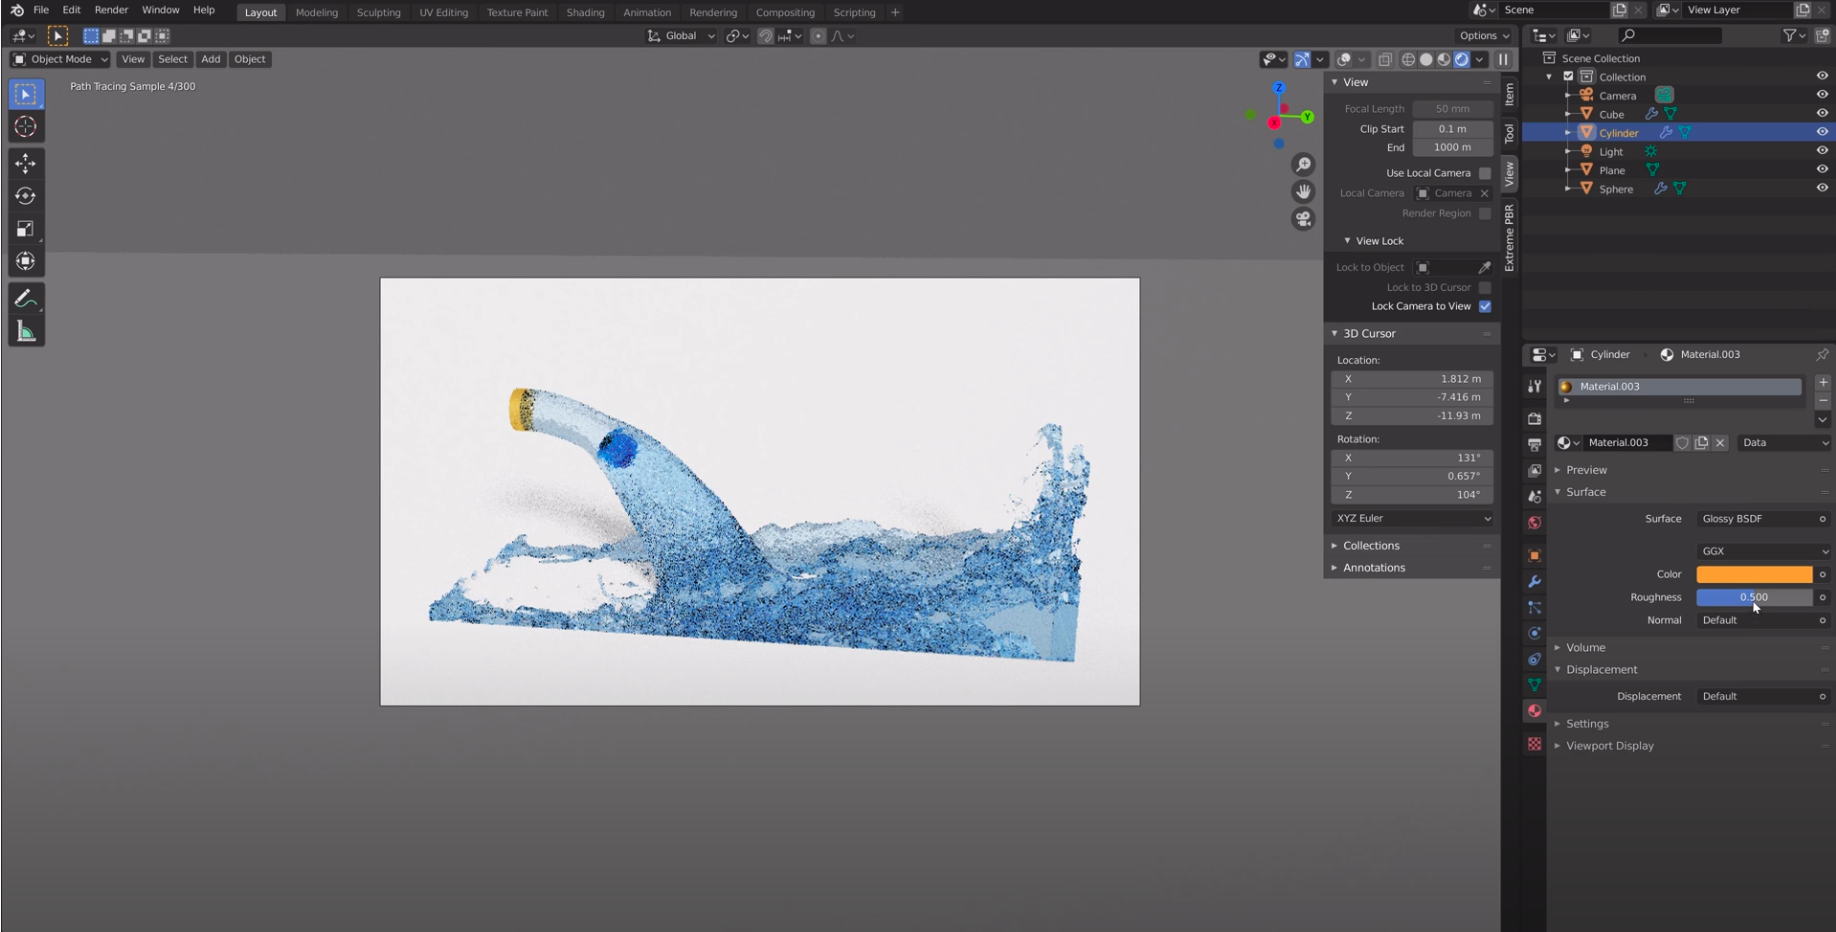
\includegraphics[scale=0.2]{img/mantaflow.png}
	\end{center}
	\captionsetup{justification=centering}
	\caption{Моделирование волн в среде Mantaflow в Blender}
	\label{img:mantaflow}
\end{figure}

В коммерческих и научных проектах используется FLOW-3D, который представляет набор инструментов для моделирования жидкостей, с целью исследования динамики их движения. Данный пакет позволяет моделировать линейные и нелинейные распространяющиеся поверхностные волны. На рисунке \ref{img:flow-3d} показаны линейный волны, визуализированные в FLOW-3D.

\begin{figure}[H]
	\begin{center}
		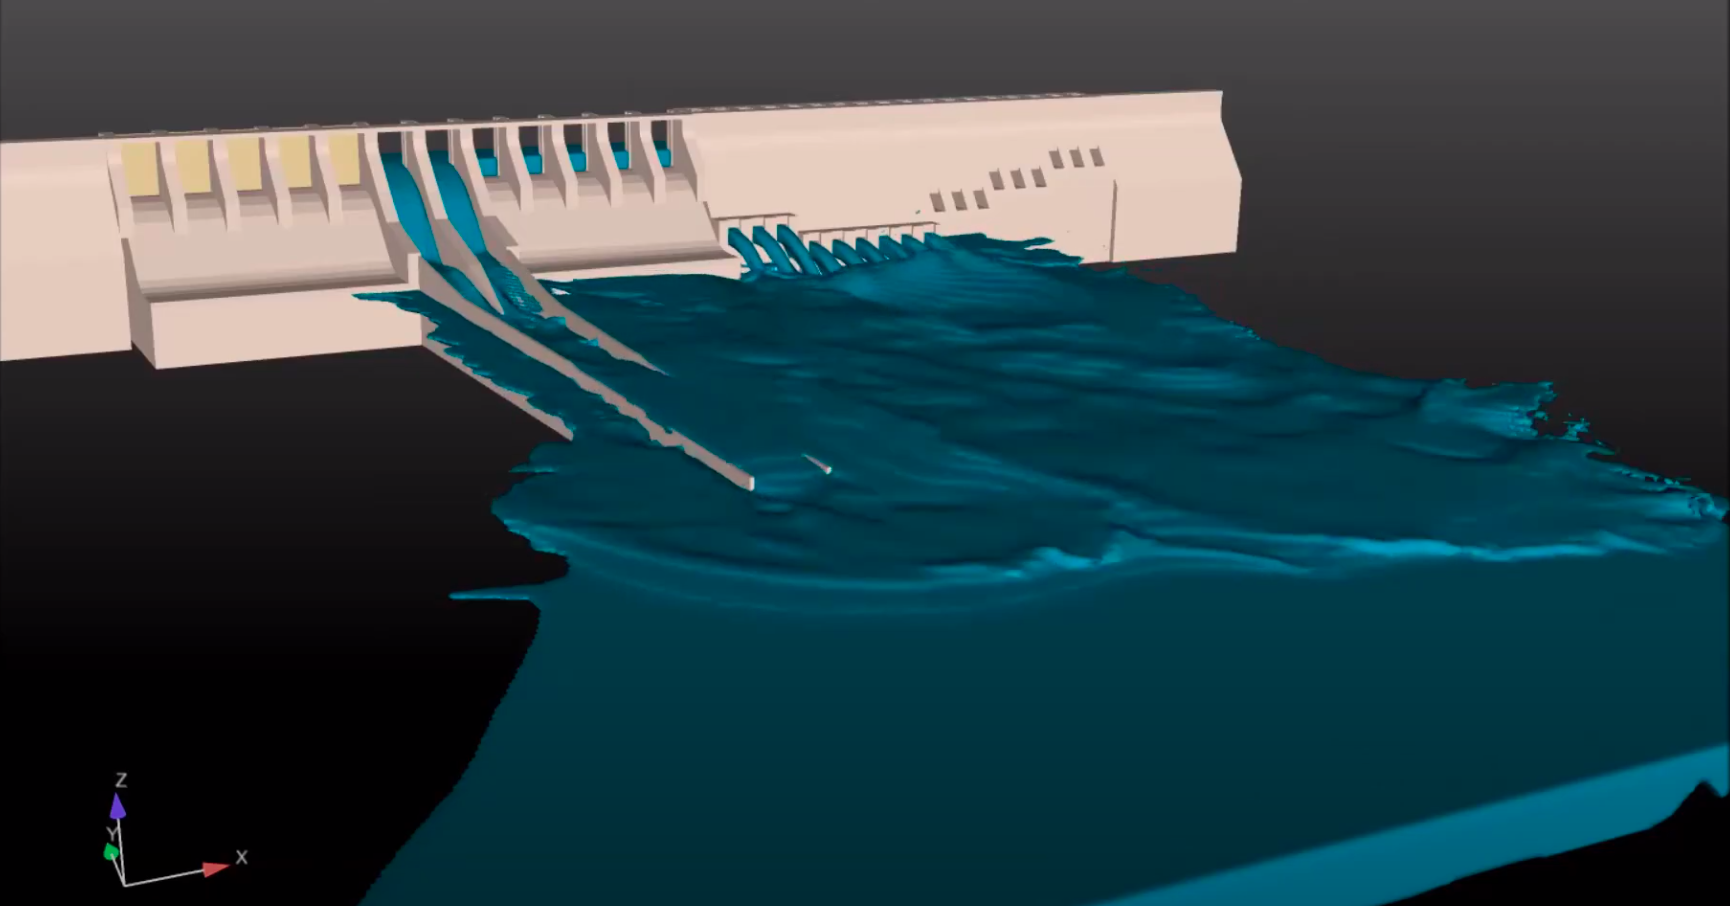
\includegraphics[scale=0.2]{img/flow-3d.png}
	\end{center}
	\captionsetup{justification=centering}
	\caption{Моделирование волн при помощи пакета FLOW-3D}
	\label{img:flow-3d}
\end{figure}

\section*{Вывод}

В ходе изучения волнового процесса были рассмотрены модели волны и предмета. Было проведено сравнение методов и алгоритмов, моделирующих волны. В качестве метода визуализации был выбран метод поля высоты, в качестве метода рендеринга изображения --- OpenGL.